Si el ratón está sobre un objeto gráfico, podemos pulsar alguna tecla para realizar una acción. Por ejemplo podemos enmudecer un clip de audio, o modificar la ganancia de una pista. Un comando de teclado es una pulsación simple de tecla, una combinación de teclas, o un movimiento de ratón mientras se mantiene pulsada una tecla. Seguidamente se muestra la notación empleada para las distintas categorías de acciones de teclado, y cómo se ejecutan.

\begin{description}
\item[Acción de teclado sencilla \sact{K} -- Pulsar y soltar:]
Se interpreta como: ``Pulsar y soltar la tecla'', como cuando escribimos una letra.
``K'' es la tecla a usar (\emph{Nota:} Aunque escribimos letras mayúsculas en la notación, simplemente hay que pulsar la tecla ``K'' sin usar nunca las teclas de mayúscula o bloqueo de mayúsculas, a menos que se indique lo contrario). Por ejemplo:
\begin{quotation}
   \sact{F}
\end{quotation}
significa pulse y suelte la tecla ``F''.

\item[Acción de teclado sencilla \hact{K} -- Pulsar y mantener:]
Se interpreta como: ``Pulsar y mantener la tecla''. En un editor de texto, obtendría muchas kkkkkkkkkkk\dots.
Nuevamente, ``K'' es la letra asociada a la acción. Por ejemplo:
\begin{quotation}
   \hact{D}
\end{quotation}
significa presione y mantenga la tecla ``D''.

Por sí mismo, el mantener una tecla pulsada no hace nada. Pero si mueve el ratón mientras una tecla está pulsada, se puede realizar una ``acción analógica''. Por ejemplo mover un clip de audio.

\item[Acción de teclado sencilla \dact{K} -- Pulsar y soltar dos veces:]
Se interpreta como: ``Presione y suelte la tecla dos veces''. Como teclear una letra dos veces, bastante rápido, a la velocidad de un doble click. Por ejemplo:
\begin{quotation}
   \dact{G}
\end{quotation}
significa presionar y soltar la tecla ``G'' dos veces.

\item[Acción de teclado doble \sact{K K} -- Pulsar y soltar:]
Se interpreta como:``Pulse y suelte dos teclas a la vez''. Es una de las acciones más difíciles. Por ejemplo:
\begin{quotation}
   \sact{F G}
\end{quotation}
significa pulsar y soltar las teclas ``F'' y ``G'' a la vez.

\item[Acción de teclado doble \hact{K K} -- Pulsar y mantener:]
Se interpreta como ``Presione y mantenga dos teclas a la vez''. Por ejemplo:
\begin{quotation}
   \hact{F G}
\end{quotation}
significa presionar y mantener las teclas ``F'' y ``G'' a la vez.

Sigue el mismo patrón que la ``Acción de teclado sencilla: pulsar y mantener'', aunque presionando dos teclas. Es un poco más difícil de realizar que con una sola tecla, y en general se reserva para acciones avanzadas.

\item[Acción de teclado doble \dact{K K} -- Pulsar y soltar dos veces:]
Se interpreta como: ``Pulse y suelte ambas teclas dos veces''. Es una acción difícil de ejecutar. Las dos teclas deben pulsarse y soltarse al mismo tiempo, dos veces. y bastante rápido. Por ejemplo:
\begin{quotation}
   \dact{F G}
\end{quotation}
significa pulsar y soltar las teclas ``F'' y ``G'' a la vez, dos veces.

De hecho, este comando no se usa mucho debido a su dificultad de ejecución, pero eso mismo lo convierte en un candidato perfecto para acciones destructivas.
\end{description}

El cursor indica qué tipo de objeto va a recibir la acción de teclado, mostrando una letra cerca del símbolo del cursor. Cuando estamos sobre una pista aparece una T, sobre un clip una C, sobre un fade una F, y sobre un plugin una P (\FigB~\ref{fig_cursor}). Si la acción de teclado no es aplicable al objeto activo, la acción se transmite al objeto que esté debajo. Por ejemplo en el caso de \hact{D} sobre un fade, la acción es enviada al clip de audio en el que está el fade.

Desde el menú ``Ajustes $\rightarrow$ Preferencias\dots'', en la página ``teclado'', pulsando los botones ``Exportar teclado'' o ``Imprimir teclado'', puede exportar el mapa de teclado. Esto permite tener siempre a la vista el mapa de teclado actualizado.

\begin{figure}[htb]
 \centering
 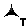
\includegraphics[height=2\baselineskip]{../images/cursorFloatOverTrack.png}\qquad
 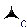
\includegraphics[height=2\baselineskip]{../images/cursorFloatOverClip.png}\qquad
 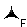
\includegraphics[height=2\baselineskip]{../images/cursorFloatOverFade.png}\qquad
 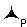
\includegraphics[height=2\baselineskip]{../images/cursorFloatOverPlugin.png}
 \caption{Según el tipo de objeto sobre el que esté el cursor, a su lado aparece una letra diferente. De izquierda a derecha: Pista, Clip, Fade, Plugin.}
 \label{fig_cursor}
\end{figure}
